\subsection{MNIST}\label{mnist}
The ``Modified National Institute of Standards and Technology'' dataset \citep{mnist} comprises a collection of 70,000 handwritten digits carefully divided into a training set of 60,000 images and a test set of 10,000 images. Each digit is represented in a grayscale image of 28$\times$28 pixels, and offers a wide range of styles and shapes. This dataset is widely recognized for its simplicity and effectiveness in benchmarking classification algorithms, making it an ideal starting point for those new to deep learning. Some examples of the dataset can be seeen in Figure~\ref{fig:MNIST}

\begin{figure} [ht]
    \centering
    
\includegraphics[width=.8\textwidth]{figures/MNIST.png}
    \caption{Example grayscale images of the MNIST dataset}\label{fig:MNIST}
\end{figure}

\subsection{MedMNIST}\label{medmnist}

MedMNIST, a more specialized and challenging dataset than MNIST, is tailored for medical image classification tasks. It extends the concept of handwritten digit classification to a diverse range of medical imaging modalities, including dermatology or radiology. Unlike MNIST's uniform format, MedMNIST encompasses 12 subsets for 2D and 6 subsets for 3D data. For our project, we focused on the PathMNIST \citep{kather2018, kather2019} subset, which includes ``100,000 non-overlapping image patches from hematoxylin and eosin stained histological images, and a test dataset [$\ldots$] of 7,180 image patches from a different clinical center'' \citep{medmnistv1}. The images could be classified into nine different types of tissues.

Initially, the images were of high resolution (3 $\times$ 224 $\times$ 224 pixels), but the authors of MedMNIST resized them to 3 $\times$ 28 $\times$ 28 pixels. The 100,000 training images were then originally divided into training and validation sets in a 9:1 ratio. Some examples of the various images can be seen in Figure~\ref{fig:MedMNIST}.

\begin{figure}[ht]
    \centering
    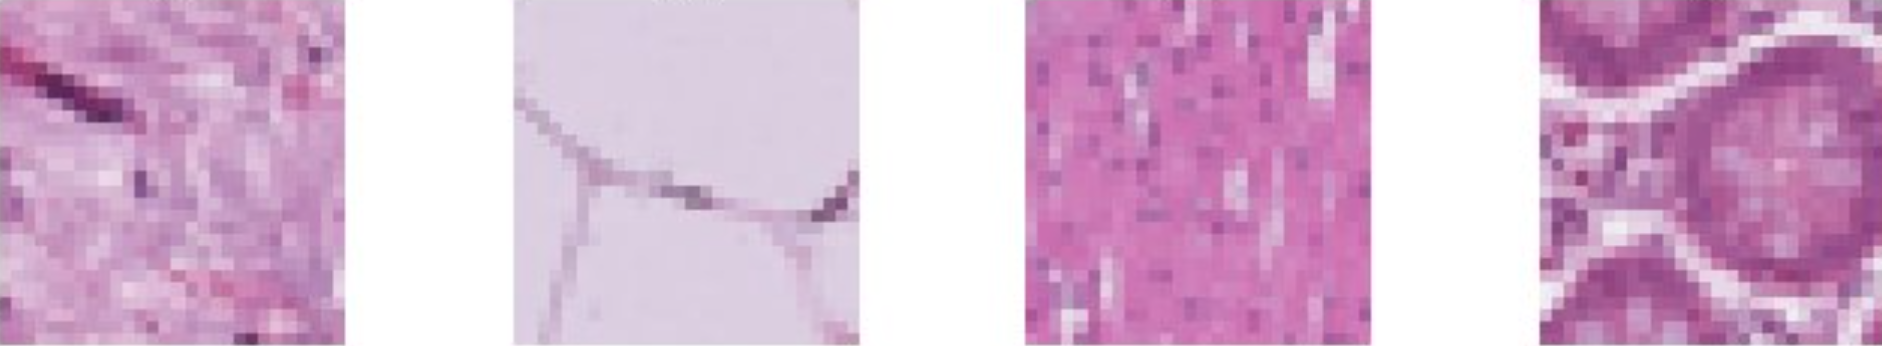
\includegraphics[width=.8\textwidth]{figures/MedMNIST.png}
    \caption{Example images of the MedMNIST dataset.}\label{fig:MedMNIST}
\end{figure}


The PathMNIST subset provides a unique challenge by introducing the complexity of medical image analysis. It requires the use of advanced deep learning techniques and models to accurately classify different types of tissue, making it an excellent progression from the simpler MNIST dataset.
